% This is samplepaper.tex, a sample chapter demonstrating the
% LLNCS macro package for Springer Computer Science proceedings;
% Version 2.21 of 2022/01/12
%
\documentclass[runningheads]{llncs}
%
\usepackage[T1]{fontenc}
% T1 fonts will be used to generate the final print and online PDFs,
% so please use T1 fonts in your manuscript whenever possible.
% Other font encondings may result in incorrect characters.
%
\usepackage{graphicx}
% Used for displaying a sample figure. If possible, figure files should
% be included in EPS format.
%
% If you use the hyperref package, please uncomment the following two lines
% to display URLs in blue roman font according to Springer's eBook style:
%\usepackage{color}
%\renewcommand\UrlFont{\color{blue}\rmfamily}
%
\usepackage[ngerman]{babel}
\usepackage{wrapfig}
\usepackage{graphicx}
\usepackage{algorithm2e}
\usepackage{floatflt}
\RestyleAlgo{ruled}
\begin{document}
%
\title{Gruppe 3 - mehrschichtige und dezentrale Entscheidungsprozesse in Agentensystemen}
\pagenumbering {gobble}
%
%\titlerunning{Abbreviated paper title}
% If the paper title is too long for the running head, you can set
% an abbreviated paper title here
%
\author{Heinz Stadler\and
Melinda Betz\and
Phil Heger\and
Björn Wladasch}
%
\authorrunning{H. Stadler et al.}
% First names are abbreviated in the running head.
% If there are more than two authors, 'et al.' is used.
%
\institute{FernUniversität in Hagen, Universitätsstraße 47, 58097 Hagen, Deutschland
\email{\{vorname.nachname\}@studium.fernuni-hagen.de}\\
\url{https://www.fernuni-hagen.de}}
%
\maketitle              % typeset the header of the contribution
%
%
\section{Einleitung}
Der MAPC \textit{Multi-Agent Programming Contest} 2021\cite{MAPC2021} bildet die thematische Grundlage für die in diesem Dokument beschrieben Agentensysteme. Es handelt sich um zwei Varianten, basierend auf der BDI-Architektur \cite{Bratman1987}, die das menschliche Denken und Schlussfolgern abstrahiert bzw. nachbildet. Beide Konzepte, nachfolgend als Agentensystem V1 (siehe Kap. \ref{agentV1}) bzw. V2 (siehe Kap. \ref{agentV2}) bezeichnet, unterscheiden sich konzeptionell durch unterschiedlich stark zentralisierte Entscheidungsprozesse.
Die Gruppe erhoffte sich durch das Verfolgen verschiedener Ansätze differenzierte Lösungen von Teilproblem, deren Vor- und Nachteile gegenseitig abgewogen werden sollten.


Als Grundlage diente das \textit{javaagents} Gerüst der MASSim (\textit{Multi-Agent Systems Simulation Platform}) \cite{EISMASSim} in der Sprache Java. Die Entscheidung für eine universelle Programmiersprache basierte auf dem Wunsch nach umfangreichen Werkzeugen und Bibliotheken zur Verifikation und Problemfindung und wurde durch die Aussage von T. Albrecht, dass für viele Teilnehmer am MAPC \textit{Multi-Agent Programming Contest} die Fehlerfindung eine schwierige und zeitintensive Aufgabe darstellt \cite[S. 17]{Ahlbrecht2021}, untermauert.

Die Konzeption der Agentensysteme erfolgte mittels UML-Diagrammen in gemeinsamer Gruppendiskussion.
Der Entwicklungsprozess wurde über das Versionsverwaltungssystem \textit{Github} und dessen Aufgaben- bzw. Fehlermanagement gesteuert. Es wurden Aufgaben ermittelt, Bearbeiter zugewiesen und für jede Aufgabe einzelne \textit{Feature-Branches} erstellt. Vor der Integration in den Hauptstamm des Quellcodes wurden die Änderungen durch ein weiteres Gruppenmitglied überprüft und anschließend freigegeben. Dieser Prozess soll Qualität des Quelltextes erhöhen, sowie das gemeinsame Verständnis fördern.


\section{Agentensystem V1 - Gruppenbeitrag Heinz Stadler}\label{agentV1}
Die Analyse der Ergebnisse des \textit{15. Multi-Agent Programming Contest} \cite{Ahlbrecht2021} ergab, dass nicht nur die Entscheidungsfindung der Agenten eine Herausforderung darstellt, sondern ebenso der Aufbau einer konsistenten und umfangreichen Wissensbasis (vgl. \cite[S. 29]{Ahlbrecht2021}) sowie die effiziente Problemfindung (vgl. \cite[S. 17]{Ahlbrecht2021}). \\
Als Folge dessen erfolgte der Aufbau und die Verifikation einer Wissensverwaltung (siehe \ref{wissensverwaltung}), die eine Datenstruktur zur Speicherung der Simulationsinformationen, sowie eine Lösung zum Aufbau einer globalen Karte des Simulationsgebiets umfasst. Zusätzlich wurde an der Konzeptionierung des Agentensystem V1 (siehe \ref{archAgentV1}) und dessen Ziel- und Absichtsfindung, sowie der Implementierung einer intelligenten Wegfindung (siehe \ref{wegfindung}) gearbeitet. Zur effektiven Verifizierung der Ergebnisse erfolgte die Erstellung eines grafischen Analysewerkzeugs (siehe \ref{verifikation}).
 
\subsection{Architektur}\label{archAgentV1}
Das Agentensystem V1 erweitert das BDI-Konzept \cite{Bratman1987} um zusätzliche Daten-, Berechnungs- und Entscheidungsebenen, die in Abb. \ref{g3:architecture} illustriert sind. Die zusätzlichen Entscheidungsebenen erweitern den BDI-Agenten zu einer bidirektionalen vertikalen Schichtarchitektur \cite[S. 61-62]{Weiss2000}, auf die in Abschnitt \ref{absichtsfindung} näher eingegangen wird.


\begin{wrapfigure}[13]{r}{0.4\linewidth}
\vspace{-8mm}
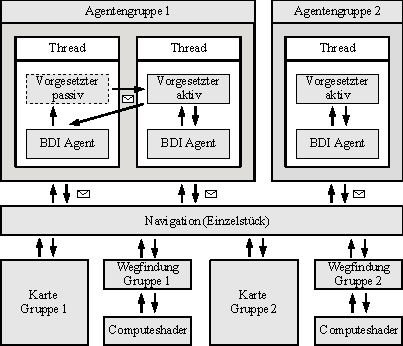
\includegraphics[scale=0.7]{./Referenzen/Architekturdiagramm.pdf}
\caption{Architektur Agent V1}
\label{g3:architecture}

\end{wrapfigure}

Jeder Agent wurde mit einer Vorgesetzteninstanz, die eine zusätzliche Entscheidungsebene bildet, kombiniert und in einem Thread parallelisiert. Werden Agenten zu einer Gruppe zusammengeführt, bleibt eine Vorgesetzteninstanz aktiv. Die sonstigen Instanzen der Gruppe werden passiv und übernehmen im Weiteren nur noch die Weiterleitung von Nachrichten an die aktive Entität.

Die Kommunikation zwischen Instanzen in verschiedenen Threads erfolgt über Nachrichten, die in einer threadsicheren Warteschlange zwischengespeichert werden. Die Verständigung des Agenten mit seinem direkten Vorgesetzten wird mittels Methodenaufrufen realisiert.

Agentengruppen aktualisieren eine gemeinsame Karte mit im Simulationsverlauf erhaltenen Umgebungsinformationen. Die Karten werden zusammen mit dem Modul zur Wegfindung von einem zentralem, threadsicheren Navigationsmodul, das als Einzelstück ausgeführt wurde, verwaltet. 


\subsection{Wissensverwaltung}\label{wissensverwaltung}
Jeder Agent hat Zugriff auf eine individuelle Wissensbasis (\textit{Beliefs}), die von der Simulation bereitgestellte Informationen auswertet und speichert.
Die aus dem Sichtfeld des Agenten erhaltenen partiellen Umgebungsdaten werden an das Navigationsmodul weitergeleitet und in einer chronologisch fortgeschriebenen Karte zusammengeführt.

Beim Simulationsstart erhält jeder Agent eine Karte mit festgelegter Initialgröße (Abb. \ref{Karte} Abschn. 1), die beim Erkunden der Umgebung erweitert wird (Abb. \ref{Karte} Abschn. 2). Treffen sich zwei Agenten aus unterschiedlichen Gruppen, wird dies vom Navigationsmodul erkannt und an die aktiven Vorgesetzten beiden Gruppen gemeldet. Stimmen beide Vorgesetzte einer Vereinigung zu, werden deren Karten überlagert (Abb. \ref{Karte} Abschn. 3) und schließlich zusammengeführt (Abb. \ref{Karte} Abschn. 4). Die entstandene Karte ermöglicht nun im weiteren Simulationsverlauf die aktuelle Position aller Agenten einer Gruppe untereinander zu bestimmen. Aus dieser Information kann durch jeweils zwei Agenten, die sich in entgegengesetzte Richtungen bewegen und sich durch die periodische Randbedingung \cite{Bungartz2013} des Simulationsgebiets zwangsläufig wieder treffen, die Kartengröße ermittelt werden. Nach erfolgreicher Ermittlung wird die Karte beschnitten, wobei die Informationen abgeschnittener Bereiche auf der gegenüberliegenden Seite eingefügt werden und somit nicht verloren gehen (Abb. \ref{Karte} Abschn. 5).
\vspace{-3mm}
\begin{figure}[h]
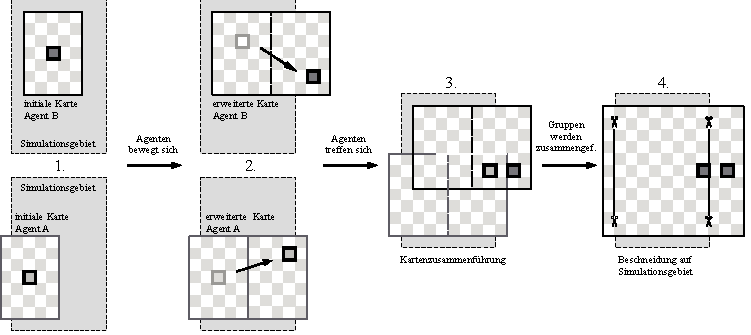
\includegraphics[scale=0.8]{./Referenzen/Kartenmerge.pdf}
\caption{Die Karte im Simulationsverlauf}
\label{Karte}
\end{figure}

\vspace{-8mm}
\subsection{Wegfindung}\label{wegfindung}
Unter dem Begriff Wegfindung verstehen wir die Berechnung des Abstands, unter Berücksichtigung von Hindernissen, zwischen zwei Punkten im Simulationsgebiet, sowie das Finden eines idealen, kürzesten Wegs zwischen diesen.

\begin{wrapfigure}[13]{r}{0.23\linewidth}
\vspace{-5mm}
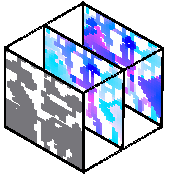
\includegraphics{./Referenzen/Pathfinding.pdf}
\caption{Datenstruktur Wegfindung (aus realer Simulation)}
\label{pathfinding}
\end{wrapfigure}

Zur Lösung der Probleme wurden klassische Suchalgorithmen wie z.B. A* \cite{Hart1968} als auch dynamische Echtzeitalgorithmen \cite[S. 182-191]{Weiss2000} untersucht. Da dynamische Algorithmen nicht zur Entfernungsermittlung eingesetzt werden können, wurde sich für den A* Algorithmus mit Heuristik Manhattan-Distanz \cite{Craw2017} entschieden.

Durch geschätzte 50-100 Berechnungen pro Agent und Simulationsschritt schied eine CPU-basierte Lösung aufgrund Zeitbeschränkungen in der Absichtsfindung aus. Es erfolgte die Implementierung des Suchalgorithmus in der Form eines \textit{Computeshaders} in der GLSL (\textit{OpenGL Shading Language}) \cite{GLSL}. Mit dieser Technologie konnte die Wegfindung auf über 1000 Berechnungen pro Simulationsschritt in praktikabler Berechnungszeit\footnote{ca. 20-250 ms auf einer integrierten Intel UHD Graphics 620 Grafikkarte} parallelisiert werden.

Als Ein- und Ausgabedatenstruktur wurde eine 3D-Textur (siehe Abb. \ref{pathfinding}) gewählt, die zusätzlich als visuelle Hilfestellung bei der Problemfindung diente und sowohl die Eingabekarte codiert als auch die Berechnungsergebnisse aufnimmt.

Bei der Wegberechnung wird das Überqueren von mit Hindernissen belegten Zellen mit zusätzlichen Kosten bewertet. Die Agenten erhalten somit einen kürzesten Weg, der sowohl Wege durch Hindernisse, als auch Wege um diese herum enthalten kann.

\subsection{Ziel- und Absichtsfindung}\label{absichtsfindung}
Die Ziel- und Absichtsfindung erfolgt über zwei Ebenen in einer vertikalen bidirektionalen Schichtarchitektur aus einem BDI-Agenten und dessen Vorgesetzteninstanz (Abb. \ref{absichtsfindung}). Der Agent ist in der Lage, für sich als Individuum, sinnvolle Ziele zu entwickeln. Die Vorgesetzteninstanz kümmert sich um die Koordinierung von Agenten zur Bewältigung von Gruppenzielen. Die Kommunikation erfolgt sowohl vom Agenten zur Vorgesetzeninstanz als auch in entgegengesetzter Richtung.


\begin{figure}[h]
\vspace{-3mm}
\centering
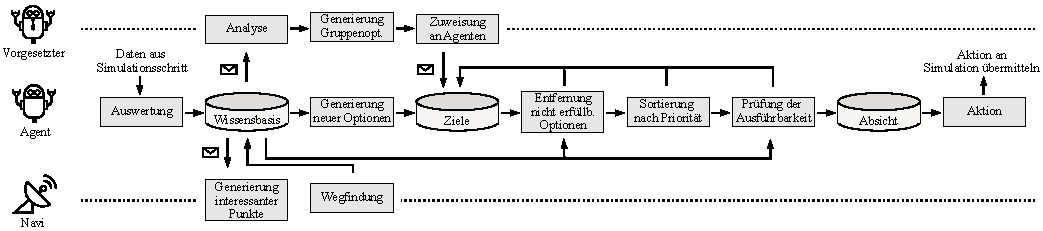
\includegraphics[scale=0.7]{./Referenzen/Entscheidungsfindung2.pdf}
\caption{Diagramm Ziel- und Absichtsfindung Agent V1}
\label{desires}
\end{figure}
\vspace{-3mm}

Zu Beginn jedes Simulationsschritts werden die aktuellen Simulationsdaten ausgewertet und die Wissensbasis der Agenten aktualisiert. Umgebungsinformationen werden an das Navigationsmodul weitergeleitet, das diese speichert und Zielpunkte für die Wegführung generiert. Zeitgleich sendet der Agent einen Ausschnitt seines aktuellen Zustands an seine Vorgesetzteninstanz. Diese versucht aus allen Agenten in der Gruppe effektive Kombinationen zu bilden, um Mehrblockaufgaben zu konstruieren, die Kartengröße zu erkunden oder die Bewachung einer Zielzone zu koordinieren.

Nachdem die Wegfindung abgeschlossen wurde, wird die Wissensbasis der Agenten aktualisiert. Im Folgenden ergänzt der Agent seine Ziele durch Optionen, die durch neue Einblock-Aufgaben entstanden sind, sowie durch Optionen die von seiner aktiven Vorgesetzteninstanz übermittelt wurden. Nicht mehr erfüllbare Optionen oder bereits erfüllte Gruppenoptionen werden anschließend aus den Zielen gelöscht.

Jede Option besitzt eine Priorität, die im Fall von Einblock-Aufgaben auch dynamisch sein kann. Der Aufbau ist modular, wodurch Optionen auch Unteroptionen enthalten können. Dies ermöglicht Teilfunktionalitäten wiederzuverwenden und die Absichtsfindung zu vereinfachen. Nach einer Sortierung gemäß Priorität wird iterativ nach ausführbaren und noch nicht erfüllten Zielen gesucht, die in eine neue Absicht umgewandelt werden. Aus der Absicht wird schließlich die nächste Agentenaktion extrahiert und an die Simulation übermittelt.

Alle bearbeiteten Optionen (über 30 Stück) sind im Paket \textit{desires} der Implementierung enthalten. Eine detaillierte Auflistung und Beschreibung überschreitet den Rahmen dieser Arbeit.


\subsection{Verifikation und Problemfindung}\label{verifikation}
Die Validierung verschiedener Strategien erfolgte über die erreichte Punktzahl in Testspielen und lieferte zufriedenstellende Ergebnisse. Die Methoden zur Verwaltung der Karte wurden mittels JUnit Tests \cite{JUnit} verifiziert. Im Gegensatz dazu konnte das Verhalten der Agenten nicht effizient durch Einzeltests verifiziert werden, da der Entscheidungsprozess in großer Abhängigkeit mit der dynamischen Wissensbasis der Agenten steht.
Als Teststrategie wurde stattdessen das genaue Beobachten der Agenten, analog eines Trainers einer Sportmannschaft, gewählt. Wurden Probleme mitverfolgt, erfolgten gezielte Einzeltests um diese zu beheben.

Dieser Ansatz erforderte zusätzliche visuelle Information, die der Monitor, über den die Simulation beobachtet werden kann, nicht liefert. Aus diesem Grund wurde ein grafisches Analysewerkzeug (siehe Abbildung \ref{debugger}), das einen detaillierten Einblick über den aktuellen Entscheidungsprozess und die Wissensbasis der Agenten liefert, implementiert. Neben allgemeiner Informationen über den selektierten Agenten werden Information über Gruppen- und Individualziele sowie Simulationsinformationen und Ergebnisse der Wegfindung angezeigt.


\begin{figure}
\vspace{-3mm}
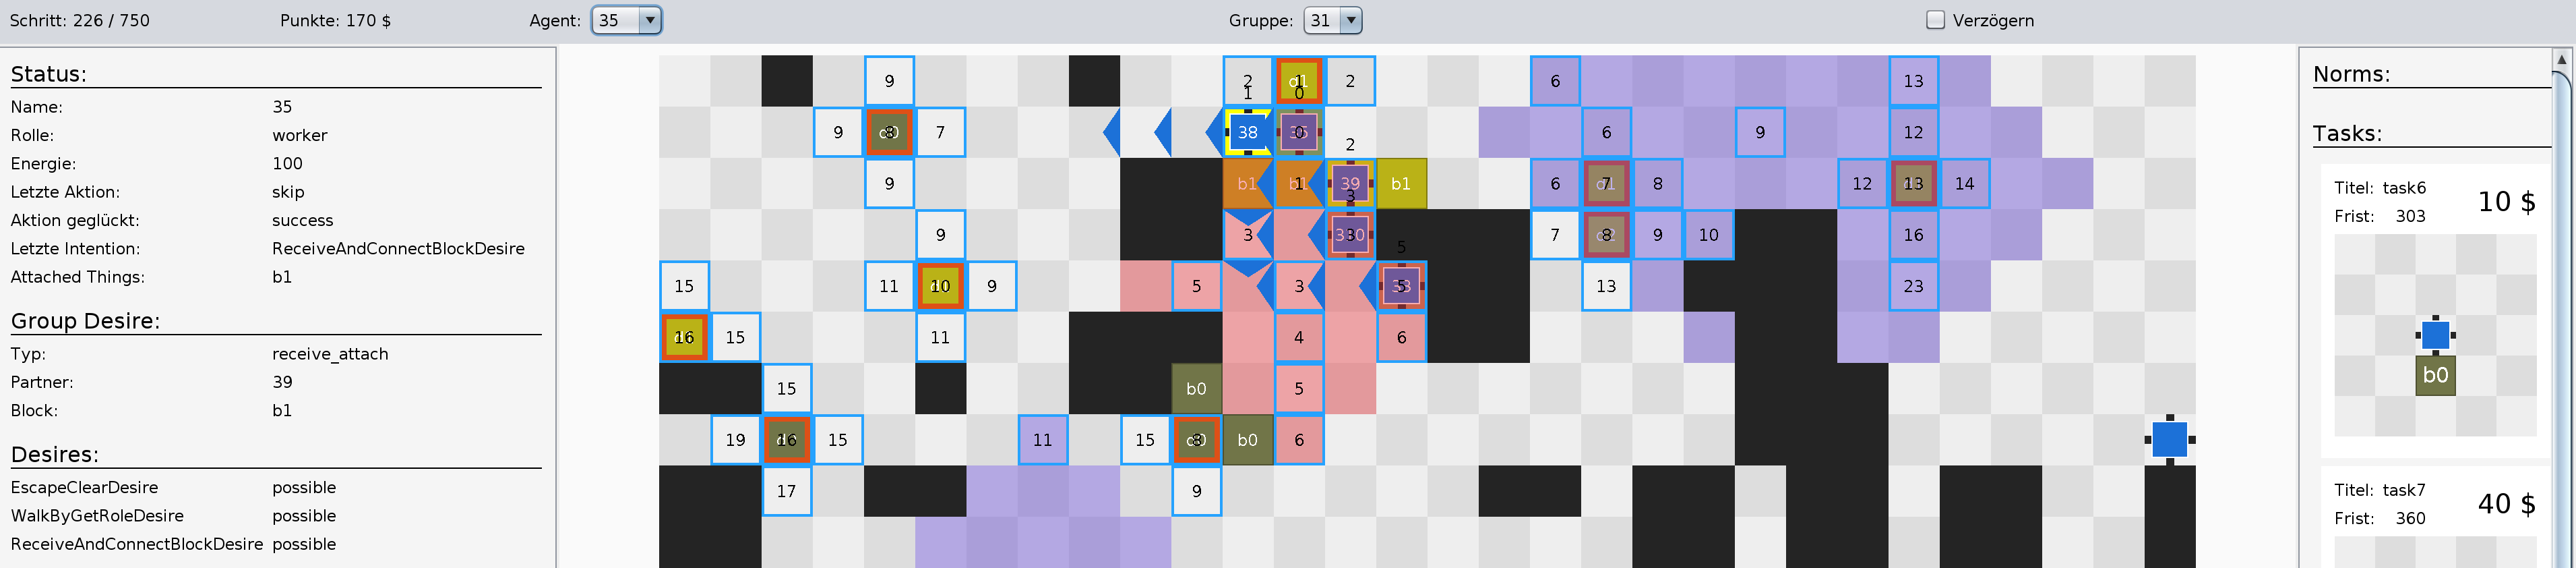
\includegraphics[scale=0.091]{./Referenzen/Debugger3.png}
\caption{Ausschnitt aus grafischem Analysewerkzeug}
\label{debugger}
\vspace{-3mm}
\end{figure}

Das Analysewerkzeug hat sich als sehr wertvoll erwiesen und ermöglichte, durch die dynamischen Echtzeitinformationen, die effiziente Weiterentwicklung der Agenten.


\section{Gruppenbeitrag Melinda Betz - Agent V2}\label{agentV2}
Neben meiner Tätigkeit als Gruppenlead habe ich einen alternativen Agenten V2 entwickelt.

\subsection{ Architektur}
Der Agent V2 arbeitet mit der Step-Methode, analog dem BasicAgent aus Massim. 
Der Agent verwendet nicht das komplette Pathfinding des V1, da OpenGL auf meinen AMD Rechnern nicht, zumindest nicht performant, funktionierte. Der Agent stellt also seine eigenen Berechnungen an, um zu einem Ziel zu kommen. Außerdem nutzt er eigene Desires, nicht die des Agenten V1. Die Desires sind dabei aufteilbar in solche, die keine Task benötigen und Desires zur Bearbeitung einer Task. Bei Letzteren ist ein Teil nur für Mehr-Block-Tasks zuständig.

\begin{description}
	\item[ohne Task]\hfill \\
	LocalExploreDesire,
	GoAdoptRoleDesire, 
	ExploreMapSizeDesire
\end{description}

\begin{description}
	\item[mit Task]\hfill \\
	GoAbandonedBlockDesire,
	GoDispenserDesire,
	GoGoalZoneDesire,
	SubmitDesire,
\end{description}

\begin{description}
	\item[Mehr\-Block\-Task]\hfill \\
	MasterMultiBlocksDesire,
	HelperMultiBlocksDesire,
	Helper2MultiBlocksDesire,
	ConnectMultiBlocksDesire,
	DisconnectMultiBlocksDesire
\end{description}

\subsection{Entscheidungsfindung}
Ein Agent durchläuft in jedem Step alle Desires und prüft ob sie in seinem momentanen Zustand (Belief) möglich bzw. ausführbar sind. Für alle ausführbaren Desires wird dynamisch, abhängig auch vom Arbeitsstand des Desires, eine Priorität vergeben. Das Desire mit der höchsten Priorität wird dann zur Intention welche in diesem Step vom Agenten ausgeführt wird.

\subsection{Strategie und Task Bearbeitung}
Wenn zwei Agenten sich treffen, schließen sie sich zu Supervisor-Gruppen zusammen, um ihr Sichtfeld zu vergrößern. Die kleinere Gruppe wird dabei in die größere integriert. Jeder Agent holt sich zuerst die Rolle Worker. Diese Rolle kann alles, manches zwar nicht ganz optimal, aber gut genug.\\

Alle Worker ohne Block besorgen sich selbständig einen Block. Um eine möglichst breite Auswahl an Blöcken zu erreichen, darf die maximale Anzahl eines Blocktyps (Setup Variable) nicht überschritten werden. Mit diesem Block bewegen sie sich in Richtung Goal Zone. Jeder Agent in einer Goal Zone, der gerade nicht an einer Mehr-Block-Task arbeitet (AgentCooperations), prüft in jedem Step für alle aktiven Tasks, ob er den innersten Block dieser Task besitzt. Eine Ein-Block-Task kann so direkt bearbeitet werden (Block in Position bringen und submitten). Für eine Mehr-Block-Task benötigt der Agent noch mindestens einen Helper, der einen weiteren passenden Block beisteuern kann, um eine neue Adhoc-Gruppe (AgentCooperation) mit sich als Master bilden zu können. In der Klasse AgentsCooperations wird festgehalten wer gerade in welcher Rolle (Master, Helper) mit welcher Task beschäftigt ist. Für alle Agenten ist dort auch der Stand der Taskabarbeitung aller anderen Beteiligten ersichtlich. Es existiert im Grunde keine zentrale Stelle zur Koordination der Agenten, jedoch gibt es einstellbare Regeln (Setup Variablen) wie viele Mehr-Block-Tasks gleichzeitig möglich sein sollen etc.. Das soll vor Klumpenbildung in der Goal Zone schützen und parallel weiterhin Ein-Block-Tasks ermöglichen.

\subsection{Umgebungsfindung und Synchronisation}
Ein Agent V2 kennt alles (vor allem Dispenser und GoalZones), was schon einmal in seinem Sichtfeld oder dem eines Agenten seiner Supervisor-Gruppe war. Entfernung und Richtung zu diesen Punkten kann er selbst ermitteln.\\

Die Synchronisation von Agenten ist, neben der beschriebenen Bearbeitung von Mehr-Block-Tasks, wichtig für die Bestimmung der Mapgröße. Dabei wird für die Ermittlung von Höhe und Breite der Map, jeweils aus den ersten beiden Treffen zweier Agenten, zentral abgewickelt über die Klasse AgentMeetings, eine AgentCooperation gebildet. Der Master läuft einmal um die Map herum. Der Helper wartet bis dieser wieder zurück ist. Aus der Position des Masters bei dem erneuten Treffen kann nun die genaue Größe (Höhe oder Breite) der Map berechnet werden. 

\subsection{Schwierigkeiten und Lösungsstrategien}
Eine Hauptschwierigkeit war, nicht genau zu wissen, was ein Agent gerade attached hat, da diese Information im Percept des Servers nicht detailliert enthalten ist. Die Lösung, sich diese Information in Variablen zu merken, funktionierte zwar prinzipiell, stieß aber spätestens bei Einführung der Clear-Events an Grenzen. Außerdem hat man Schwierigkeiten, wenn ein Agent mit einer Geschwindigkeit größer zwei läuft und in einem Schritt abbricht (Returncode partial\_fail). Es ist dann nicht möglich herauszufinden, wie weit der Agent vor dem fail gekommen ist, wo er sich also gerade auf dem Spielfeld befindet. Hier ist die etwas unbefriedigende, aber stets erfolgreiche Lösung die: kein Agent läuft schneller als zwei (was durch die Rolle Worker automatisch gegeben ist). 

\subsection{Verbesserungspotential}
Was ich noch deutlich verbessern müsste ist, wie oben schon erwähnt, zum einen die dynamischere Erkennung der Umgebung (Goal Zones, Dispenser etc.) sowie das Nachführen der Informationen über die aktuellen Attachements der Agenten. Beides ist durch meine Versuche, diese Neuerungen für Turnier 6 einzubauen, eigentlich nur schlimmer geworden und war in „älteren Agenten“ schon mal wesentlich besser.\\

Potential würde ich auch noch bei meinen oben beschriebenen AgentCooperations sehen. Diese sind derzeit, einmal angelegt, zu starr. Der Master wartet auf seine Helper geduldig bis zum Ende aller Tage, genau genommen bis zur Deadline der betroffenen Task. Eine dynamischere Variante, bei der der Master unterdessen neue Gelegenheiten mit anderen Agenten wahrnehmen kann, wäre wohl zu bevorzugen.  

\section{Gruppenbeitrag Phil Heger}
\subsection{Logging}
Anfangs wurde ein Logging-Modul (AgentLogger.java) implementiert, in dem der Logging-Output konfiguriert wird. Dieses Modul ermöglicht es, den Logging-Output, der von einem Agenten in einem bestimmten Desire oder Modul ausgegeben wird, in eine eigene Datei zu schreiben. Dadurch sind die Entscheidungsfindung dieses Agenten und seine Zustandsänderungen besser nachvollziehbar, als wenn der gesamte Logging-Output aller Agenten in der gleichen Konsole bzw. Datei ausgegeben wird und nachträglich gefiltert werden muss. 

\subsection{Strategien zum Stören gegnerischer Agenten}
Durch eine gezielte clear-Aktion auf die Position des Gegners wird dessen Energielevel um einen definierten Betrag verringert. Beträgt sein Energielevel 0, dann wird der Agent für einige Runden deaktiviert und verliert die Verbindung zu allen mit ihm verbunden Blöcken. Dabei gibt es zwei Probleme, die die Wirksamkeit einer einfachen Strategie (z.\,B. Angreifen beliebiger Agenten an beliebigen Stellen der Karte) stark verringern:
\begin{itemize}
\item{Bei der clear-Aktion muss das Feld angegeben werden, auf dem sich der gegnerische Agent am Ende der Runde befinden wird. Diese Position ist bei gegnerischen Agenten jedoch unbekannt, da er sich in alle Richtungen bewegen oder auch stehenbleiben kann. Die Wahrscheinlichkeit, den Gegner zu treffen, ist dadurch sehr gering.}
\item{Der Schaden einer erfolgreichen clear-Aktion ist nicht sehr groß. So beträgt der max. mögliche Schaden, wenn sich der angegriffene Agent in einem angrenzenden Feld befindet, nur 16\,Punkte bei einer Gesamtenergie von 100\,Punkten. Der Schaden halbiert sich mit der Distanz zum gegnerischen Agenten. Hinzu kommt, dass die Erfolgswahrscheinlichkeit der clear-Aktion bei allen Rollen (außer der Rolle \textit{digger}) nur 30\,\% beträgt.}
\end{itemize}
Für ein wirksames Stören der Gegner ist daher eine komplexere Strategie und das Annehmen der Rolle \textit{digger} erforderlich.
\subsubsection{Dispenser blockieren}
Die erste Idee besteht darin, das Sammeln von Blöcken für die gegnerischen Agenten zu erschweren, indem ein eigener Agent auf das gleiche Feld wie ein Dispenser geht und dort verbleibt. Dadurch ist es nicht mehr möglich an diesem Dispenser neue Blöcke zu erzeugen. Dabei werden Dispenser ausgewählt, die für die Bearbeitung der aktuellen Aufgaben am wichtigsten sind. Aufgrund der hohen Anzahl an Dispensern in den Tunier-Konfigurationen zeigte sich jedoch, dass dieser Ansatz nicht praktikabel ist, da eine große Anzahl an eigenen Agenten für das Blockieren der vielen Dispenser notwendig wäre. Um die eigenen Agenten nicht ebenfalls zu behindern, müssen diese über blockierte Dispenser informiert werden.

\subsubsection{Goal Zone verteidigen}
Bei diesem Ansatz wurde der in der Einleitung dieses Unterkapitels erwähnte grundlegende Mechanismus (clear-Aktion auf Position des gegnerischen Agenten) umgesetzt, wobei der eigene Agent gegnerische Agenten nur in der Zielzone angreift, da die gegnerischen Agenten hier oft auf andere Agenten warten und sich in dieser Zeit nicht bewegen. Der eigene Agent kann sich dadurch nähern und mit dem größtmöglichen Schaden angreifen. Ist der gegnerische Agent deaktiviert, werden alle mit ihm verbundenen Blöcke gelöst. Diese können anschließend vom angreifenden Agenten mit clear-Aktionen entfernt werden. Neben dem Deaktivieren des Agenten für einige Runden war auch der Aufwand des Holens der Blöcke für umsonst. Hinzu kommt die Chance, den gegnerischen Algorithmus des Zusammenbauens von größeren Aufgaben zu stören.

In der Umsetzung wurde jeder der zwei in den Turnier-Konfigurationen definierten Zielzonen ein Agent fest zugewiesen. Für eine ausreichend hohe Effektivität muss der ausgewählte Agent die Rolle \textit{digger} annehmen, damit die clear-Aktionen mit einer Wahrscheinlichkeit von 100\,\% ausgeführt werden.

Für die Umsetzung der Strategie wurden folgende Teilaufgaben gelöst:
\begin{itemize}
\item{Zuordnung eines Agenten zu jeder Zielzone}
\item{Analyse von Dingen, die mit einem Gegner verbunden sind bzw. sein könnten (direkt an ihn angrenzende, zusammenhängende Blöcke)}
\item{Auswahl eines zu attackierenden Gegners basierend auf den mit ihm verbundenen Dingen und der Distanz zu ihm}
\item{Bewegungen in der Zielzone (um Hindernisse herum, auf den Gegner zu bzw. patrouillieren, wenn sich keine geeigneten Gegner im Sichtfeld befinden)}
\item{Energie des angegriffenen Gegners mitzählen}
\item{Gegnerverfolgung (um die Energie eines Agenten mitzählen zu können und für die Verfolgung und Fortsetzung des Angriffs, wenn er sich bewegt)}
\item{Zuletzt angegriffenen Gegner merken und nicht direkt noch einmal angreifen}
\end{itemize}

Getestet wurde die Strategie, indem die eigenen Agenten auch als Gegnerteam eingesetzt wurden. Die Strategie ist nur wirksam, wenn sich gegnerische, Blöcke tragende Agenten ausreichend lange in der Zielzone nicht bewegen. Gegen 1-Block-Aufgaben ist die Strategie dadurch völlig wirkungslos, da die gegnerischen Agenten dabei in die Zielzone laufen und sofort die Aufgabe abgeben.

\subsection{Sonstiges}
Zu Beginn der Gruppenarbeit wurde eine mögliche Architektur für den Umgang mit den \textit{Desires} anhand von UML-Diagrammen entwickelt. In der Folge wurde prototypisch eine Architektur umgesetzt. Diese stellte sich jedoch als nicht praktikabel heraus, da die \textit{Desires} sehr kleinteilig aufgeteilt und in jedem Schritt die \textit{Desire}-Objekte neu erzeugt wurden und somit Zustände nicht gespeichert werden konnten. Das Konzept wurde deshalb überarbeitet.

Zwischenzeitlich wurde außerdem ein \textit{Desire} entwickelt, bei dem ein Agent eigenständig alle Blöcke für beliebig komplexe Aufgaben sammelt und zusammenbaut. Dies wurde jedoch zugunsten von kooperierenden Agenten, die sich gegenseitig Blöcke holen, abgebrochen.

\section{Gruppenbeitrag Björn Wladasch}
\subsection{Kartengrösse bestimmen}
Um dem Problem der endlosen Karte zu begegnen sollte eine Methode entwickelt werden die es ermöglicht, die tatsächliche Kartengröße zu bestimmen. Die Basisidee wie soetwas umgesetzt werden könnte, wurde der Dokumentation des letzten Wettbewerbs \cite{MAPC2021} entnommen.  

Da in der Literatur aber keine vollständige Erklärung des verwendeten Algorithmus angegeben war, wurde mit verschiedenen Ansätzen zur Bestimmung der Kartengröße experimentiert. Unter anderem wurde versucht aus dem initialen Abstand zweier Agenten, der Anzahl der gemachten Schritte (in Richtung der zu vermessenden Achse) und dem Abstand bei erneuter Sichtung des Agenten zu berechnen, wie groß die Karte ist, was aber erfolglos blieb.

Nach zahlreichen Versuchen wurde eine verlässliche Lösung gefunden, die im Folgenden vorgestellt wird.

Dazu muss man zunächst ein paar Vorbemerkungen zur Ausgangslage im betrachteten Agenten (BDIAgentV1) machen. Agenten können zu Gruppen zusammengefasst werden, welche isch danneine Karte teilen, so dass die absolute Positionen der Agenten (im Bezug auf diese Karte) bekannt sind. Mittels einer Methode des zugehörigen Kartenobjektes ist es jederzeit möglich, über den Namen eines Agenten dessen bekannte Position auf der Karte zu erhalten.

Die Koordinaten der \textit{Things}, die von den jeweiligen Agenten gesehen werden, werden in relativen Koordinaten angegeben (also dem Abstand auf der x- bzw. y-Achse) bezogen auf die Position des Agenten. Diese befindet sich immer im Zentrum seines Sichtfeldes, und hat somit die relativen Koordinaten (0,0).


Die Grundidee zur Bestimmung der Kartengröße besteht nun darin, zwei Agenten miteinander zu verbinden ( es reicht, dass ein Agent den Namen des anderen Agenten kennt) und in entgegengesetzte Richtungen loszuschicken, jeweils ein Paar ( in der Abbildung sind die beiden Agenten der Einfachheit halber mit W und E benannte) entlang der x-Achse in Richtung Westen bzw. Osten und ein Paar in Richtung Norden bzw. Süden entlang der y-Achse.

\begin{figure}
\centering
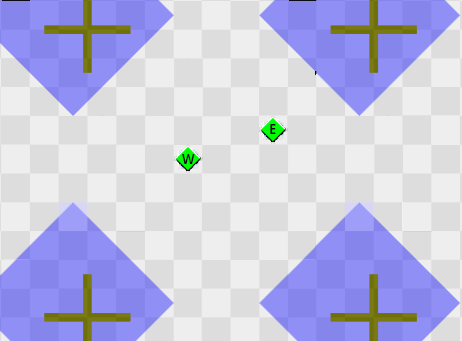
\includegraphics[scale=0.5]{./Referenzen/Measurement_Step1.png}
\caption{Startsituation}
\label{measurement1}
\end{figure}

Auf Grund der sich wiederholenden Karte muss ein Agent der nach Westen läuft zwangsweise seinem Gegenstück das nach Osten gegangen ist wieder begegnen, sobald einer der Beiden (oder beide) die Kartengrenze überschritten haben.In Nord- Süd-Richtung passiert das ganze analog und wird hier nicht weiter betrachtet.

Die mit der Kartenvermessung beauftragten Agenten betrachten nun jeden Agenten aus dem eigenen Team der vor ihnen in Bewegungsrichtung auftaucht und prüfen ob es sich um den gesuchten Agenten handelt.

Die Position diesen entdeckten Agenten (hier als U1 bzw. U2 bezeichnet) auf der gemeinsamen Karte lässt sich bestimmen, in dem die eigene Kartenposition zur relativen Position des gefundenen Agenten hinzu addiert wird. Ist dabei die y-Koordinate (im Nord-Süd-Fall die x-Koordinate) identisch mit der bekannten Position des gesuchten Agenten und die x-Koordinate (bzw. y- Koordinate im Nord-Süd-Fall) entspricht nicht der bekannten Position des gesuchten Agenten so besteht die Möglichkeit, dass der andere Agent gefunden wurde. Wenn dieser an inverser relativer Position ebenfalls einen passend Agenten sieht, haben sich die beiden Agenten wiedergefunden.

Beispiel (in Abbildung) 
Der Agent U1 ist aus Sicht von Agent W die Koordinaten (-1,-1). Aus Sicht des Agenten E hat U2 die Koordinaten (1,1), was genau die entgegengesetzten Koordinaten sind. Damit sehen die beiden Agenten W und E in dem jeweiligen Agenten U1 bzw. U2 ihr Gegenstück nach Überquerung der Kartengrenze. Die Kartenbreite ist dann | U1.x - E.x | bzw. | U2.x - W.x| .

\begin{figure}
\centering
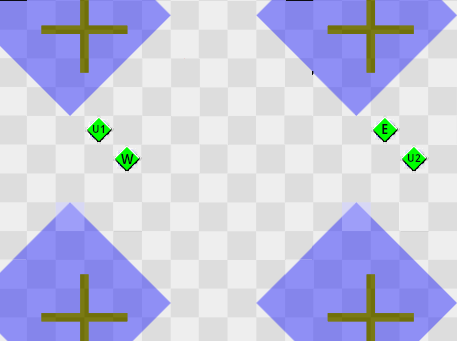
\includegraphics[scale=0.5]{./Referenzen/Measurement_Step2.png}
\caption{unbekannte Agenten gefunden}
\label{measurement2}
\end{figure}


Da auf der Karte aber zahlreiche Hindernisse im Weg der Agenten sein können, ist es wichtig, dass sich die Agenten nciht verpassen. Dazu muss man sicherstellen, dass die beiden Agenten möglichst auf einer vorher festgelegten Linie laufen, damit sie wieder in das Sichtfeld des anderen laufen. Dazu legt man einen y-Koordinaten Wert (im Fall der West- Ost-Vermessung, bei Nord -Süd Vermessung einen entsprechenden x-Wert)) fest auf den die Agenten nach Ausweichmanövern und ähnlichem immer wieder zusteuern.


\section{Turniere}\label{Turniere}
Die Gruppe nahm an den Turnieren 2-6 teil. Den Großteil der Spiele bestritt das Agentensystem V1. Das System V2 übernahm jeweils ein Spiel in den Turnieren 2-5. 

\subsection{Agent V1}
Das Agentensystem zeigte sich über alle teilgenommenen Turniere hinweg wettbewerbsfähig. Probleme in einzelnen Begegnungen wurden detailliert dokumentiert und im weiteren Entwicklungsverlauf behoben oder zumindest entschärft. Die Folgenden Absätze geben ein Überblick über die Leistung und Probleme in den einzelnen Turnieren.

\textbf{Turnier 2}
Es war erfreulich, dass 10 Agenten in der Lage waren bis zu 370 Punkte über Einblock-Aufgaben zu erringen. Trotzdem zeigte sich noch großes Verbesserungspotential bei der Befreiung von Agenten aus festgefahrenen Situationen und dem generellen Ausweichen von Agenten untereinander.

\textbf{Turnier 3}
Die erreichte Punktzahl über Einblock-Aufgaben konnte auf bis zu 720 gesteigert werden. Dies resultierte hauptsächlich aus besseren Strategien zur Befreiung aus festgefahrenen Situationen. Trotzdem waren weiterhin teilweise übermäßige Gruppenbildung und daraus resultierende gegenseitige Behinderung zu beobachten.

\textbf{Turnier 4}
Die Agenten waren erstmals in der Lage Mehrblock-Aufgaben zu bearbeiten. Das Zusammenspiel der Agenten war leider noch nicht zufriedenstellend, wodurch sich ein Rückgang der erreichten Maximalpunkte auf 680 ergab. Positiv war zu beobachten, dass die Gruppenbildung und daraus resultierender gegenseitiger Behinderung im Vergleich zum Vorturnier abgenommen hat.

\textbf{Turnier 5}
 Die Behebung eines Fehlers im Entscheidungsprozess führte zu stark verbesserter Leistungsfähigkeit und sicherte der Gruppe den Turniersieg mit maximal 1300 erreichten Punkten. In diesem Turnier wurde erstmalig in einzelnen Begegnungen aggressive Strategien gegen die gegnerischen Agenten eingesetzt.

\textbf{Turnier 6}
Das Turnier 6 bot neue Herausforderungen, da die Kartengröße nicht bekannt war, die Zielzonen sich bewegten und Meteoriteneinschläge auf der Karte ergänzt wurden. Die Agenten bewältigten die neuen Herausforderungen zufriedenstellend und konnten auch dieses Mal den Turniersieg mit einer Maximalpunktzahl von 910 sichern. Die Schwierigkeitserhöhung war deutlich in der Durchschnittspunktzahl sichtbar. Trotzdem konnten die Agenten in einzelnen Spielen die erhöhte Schwierigkeit durch die Abgabe von Dreiblock-Aufgaben kompensieren.

Interessant war weiter zu beobachten, dass speziell die Gruppe 1 sehr aggressiv gegen die Agenten vorging und dadurch eine spannende Begegnung entstand. Das Abwehren solchen Verhaltens wäre eine potenzielle Verbesserungsmöglichkeit für das Agentensystem. 

\textbf{Bonusspiel - Jeder gegen Jeden}
Zum Abschluss wurde ein Spiel mit 6 x 25 Agenten durchgeführt. Trotz der Vielzahl an gegnerischen und eigenen Entitäten zeigten sich die implementierten Strategien erfolgreich. Es wurden 1370 Punkte erreicht und das Spiel trotz erhöhter Gruppenbildung und gegenseitiger Störung mit deutlichem Abstand gewonnen.
Positiv war zu beobachten, dass die 25 Agenten weiterhin performant arbeiteten und in sämtlichen Schritten alle Instanzen eine Aktion an den Simulationsserver übermittelten.

\subsection{Agent V2}
Bei den Turnieren, mit Ausnahme von Turnier 6, sind immer beide Agenten erfolgreich zum Einsatz gekommen. Bei Turnier 6 war der Agent V2 nicht dabei, da er sowohl Probleme mit dem Erkennen der wechselnden Goal Zones hatte, vor allem mit dem Wegfall von Goal Zones, als auch mit dem Erkennen des Verlustes eines Blocks durch einen Clear-Event und so weniger Tasks als bisher erfolgreich bearbeiten konnte. Im Nachhinein wäre diese Vorsicht jedoch nicht nötig gewesen, da der Leistungsabfall zwar gegenüber dem zu diesem Zeitpunkt genialen Agenten V1 deutlich zu erkennen war, aber die anderen Gruppen anscheinend ebenfalls und mindestens so stark mit diesen neu hinzugekommen Problemen zu kämpfen hatten.

\section{Rekapitulation und Ausblick}
Die Umsetzung des erarbeiteten Wissens lieferte Lösungen, die speziell in den letzten beiden Turnieren sehr erfolgreich waren (siehe Kapitel \ref{Turniere}).


Die Entscheidung zwei Architekturansätze zu verfolgen muss kritisch bewertet werden. Beide Ansätze behinderten sich zwar nicht, es stellten sich aber leider kaum Synergieeffekt ein. Die entwickelten Ziele des Agentensystem V2 wurden auf dessen internen Aufbau optimiert und waren daher nicht für das Agentensystem V1 verwendbar. Daher blieb der erhoffte Austausch verschiedener Lösungen für das gleiche Problem unter den Systemen aus.

Sowohl der mehrschichtige Entscheidungsprozess des Agentensystems V1 als auch der komplett dezentrale Ansatz des Systems V2 lieferten funktionierende kompetitive Lösungen. Das Abschneiden in den Turnieren legt nahe, dass der mehrschichtige Ansatz Vorteile gegenüber der dezentralen Lösung birgt. Dies bleibt aber eine Vermutung, da die unterschiedlichen Entscheidungsprozesse in eigene Architekturen eingebunden sind, die den direkten Vergleich erschweren.

Die Gruppe ist mit der erreichten Funktionalität und deren Qualität zufrieden. Dennoch besteht vielfältiges Verbesserungspotential in der Entscheidungs- und Strategiefindung der Agenten.

%
% ---- Bibliography ----
%
% BibTeX users should specify bibliography style 'splncs04'.
% References will then be sorted and formatted in the correct style.
%
% \bibliographystyle{splncs04}
% \bibliography{mybibliography}
%
\begin{thebibliography}{8}
	\bibitem{Ahlbrecht2021}
	Ahlbrecht, T., Dix, J., Fiekas. N. und T. Krausburg: The Multi-Agent Programming Contest 2021, Springer, Heidelberg, 2021
	\bibitem{Hart1968}
	Hart, P. E., Nilsson, N. J. und Raphael, B.: A Formal Basis for the Heuristic Determination of Minimum Cost Paths, in IEEE Transactions on Systems Science and Cybernetics, 4. Auflage, Nummer 2, Seiten 100-107, Juli 1968
	\bibitem{Weiss2000}
	Weiss, G.: Multiagent Systems, 2. Auflage, The MIT Press, Cambridge, 2000
	\bibitem{EISMASSim}
	github.com/agentcontest/massim\_2022, agentcontest/massim\_2022, \\ https://github.com/agentcontest/massim\_2022/blob/main/docs/eismassim.md, EISMASSim Documentation, abgerufe am 21.08.2022
	\bibitem{Bratman1987}
	Bratman, M.: Intention, plans, and practical reason, Harvard University Press, Cambridge, 1987
	\bibitem{GLSL}
	Kessenich, J., Baldwin, D., Rost, R.: The OpenGL® Shading Language, Version 4.60.7, https://registry.khronos.org/OpenGL/specs/gl/GLSLangSpec.4.60.pdf, abgerufen am 10.09.2022
	\bibitem{JUnit}
	JUnit 5, https://junit.org/junit5, abgerufen am 11.09.2022
	\bibitem{Github}
	Projekt-Quellcodeverwaltung, https://github.com/h1Modeling/ss22\_fp\_mapc\_gruppe3, abgerufen am 11.09.2022
	\bibitem{Site}
	Projekt-Webseite: https://github.com/h1Modeling/ss22\_fp\_mapc\_gruppe3/tree/ master/site/index.html, abgerufen am 13.09.2022
	\bibitem{Bug}
	Massim 2022 - Issue 7: https://github.com/agentcontest/massim\_2022/issues/7, abgerufen am 11.09.2022
	\bibitem{Goal}
	GOAL: https://goalapl.atlassian.net/wiki/spaces/GOAL/overview, abgerufen am 13.09.2022
	\bibitem{MAPC2021}
	Ahlbrecht,T. , Dix, J. , Fiekas, N. ,Krausburg T. (Eds.): JaCaMo Builders: Team Description for the Multi-agent Programming Contest 2020/21  in The Multi-Agent Programming Contest 2021 One-and-a-Half Decades of Exploring Multi-Agent Systems, Springer Verlag, 2021, Seite 136
	\bibitem{Bungartz2013}
	Bungartz, H.J., Zimmer, S., Buchholz, M., Pflüger, D.: Modellbildung und Simulation Eine anwendungsorientierte Einführung, 2. Auflage, Springer Spektrum, Berlin Heidelberg, 2013
	\bibitem{Craw2017}
Craw, S.: Manhattan Distance in Encyclopedia of Machine Learning and Data Mining, Springer, Bosten, 2017, Seite 790-791	
\end{thebibliography}
\end{document}
